\section{Results}

We implement our \gls{rsp} algorithm on the aforementioned conceptual aircraft design problem.
Our objective function is total fuel consumption, which is
to be minimized given a payload and range requirement.

\subsection{Mitigation of probability of failure}

First, the optimization problem is solved in presence of no uncertainty. It is expected
that this aircraft has a high probability of failure due to its sensitivity
to the outcomes of uncertain parameters. Then, using the sign of
sensitivities of the nominal solution, we assign $3\sigma$ margins for each parameter
and generate a design using margins. These two solutions are compared with \gls{ro} results for
box and elliptical uncertainty sets at $\Gamma = 1$. From here onward we refer to
aircraft designed under margins, under box uncertainty and
under elliptical uncertainty as `the margin aircraft', `the box aircraft' and `the elliptical aircraft' respectively.

The design variables are then fixed for each solution, and the designs are simulated for
different realizations of the uncertain parameters.
This allows for statistical analysis of design performance, and
an estimate of each design's probability of constraint
violation, which we define as its probability of failure.
In this~\gls{mc} scheme, the random variables
are simulated from independent and identically distributed $3\sigma$ truncated Gaussians.
We simulate from the truncated Gaussian since this makes it possible to
confirm mathematically that for $\Gamma = 1$, all simulations of $3\sigma$ uncertain parameters are
deterministically feasible for the box uncertainty set. The results are in Table~\ref{tab:uncertainties}.
Designs for each solution
are simulated with the same set of uncertainty realizations for consistency.

\begin{table}[!h]
\begin{center}
\caption{\label{tab:results} SP Aircraft Optimization Results, for $\Gamma = 1$}
\begin{tabular}{C{2cm} C{3.8cm} C{1.25cm} C{1.6cm} C{1.6cm} C{1.6cm} C{1.6cm}}
\hline
Free variable & Description & Units & No Uncert. & Margins & Box & Elliptical \\
\hline
$L/D$ & mean lift-to-drag ratio & - & 33.4 & 23.4 & 24.8 & 27.5 \\
$AR$ & aspect ratio & - & 24.2 & 13.0 & 12.8 & 16.1 \\
$Re$ & Reynolds number & - & $1.56 \times 10^6$ & $2.69 \times 10^6$ & $3.08\times 10^6$ & $2.53 \times 10^6$ \\
$S$ & wing planform area &$\mathrm{m^2}$ & 13.6 & 32.9 & 32.1 & 28.2 \\
$\tau$ & airfoil thickness ratio & - & 0.2 & 0.2 & 0.2 & 0.2 \\
$V$ & mean flight velocity &$\mathrm{m/s}$ & 41.7 & 37.4 & 39.1 & 38.5 \\
$T_{\rm{flight}}$ & time of flight & $\mathrm{hr}$ & 20.0 & 22.3 & 21.4 & 21.7 \\
$W_{\rm{w}}$ & wing weight & $\mathrm{N}$ & 2840 & 4790 & 4820 & 4510 \\
$W_{\rm{w,strc}}$ & wing structural weight &$\mathrm{N}$ & 2020 & 2610 & 2690 & 2640 \\
$W_{\rm{w,surf}}$ & wing skin weight &$\mathrm{N}$ & 818 & 2170 & 2130 & 1870 \\
$W_{\rm{fuse}}$ & fuselage weight &$\mathrm{N}$ & 250 & 314 & 288 & 279 \\
$V_{\rm{f,avail}}$ & total fuel volume & $\mathrm{m^3}$ & 0.0765 & 0.148 & 0.156 & 0.137 \\
$V_{\rm{f,fuse}}$ & fuselage fuel volume & $\mathrm{m^3}$ & 0.0396 & 0 & 0 & 0.0156 \\
$V_{\rm{f,wing}}$ & wing fuel volume &$\mathrm{m^3}$ & 0.0368 & 0.169 & 0.166 & 0.121    \\
& sketches to scale & &
    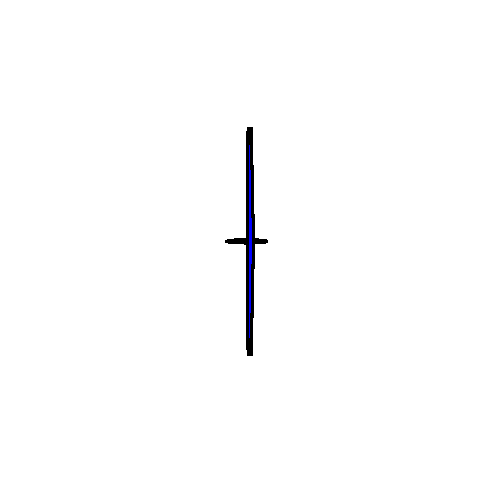
\includegraphics[trim={9.5cm 1cm 9.5cm 1cm},clip,height=3.8cm]{nominal.eps} &
    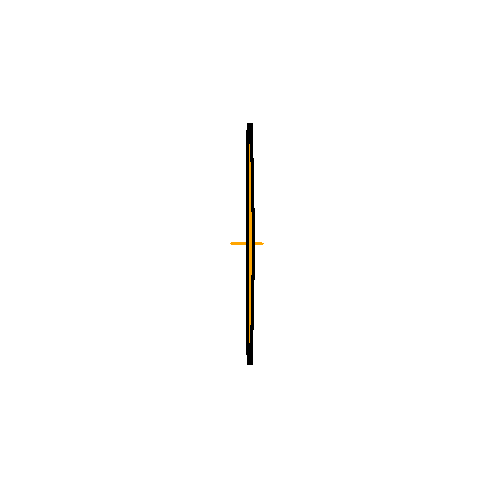
\includegraphics[trim={9.5cm 1cm 9.5cm 1cm},clip,height=3.8cm]{margins.eps} &
    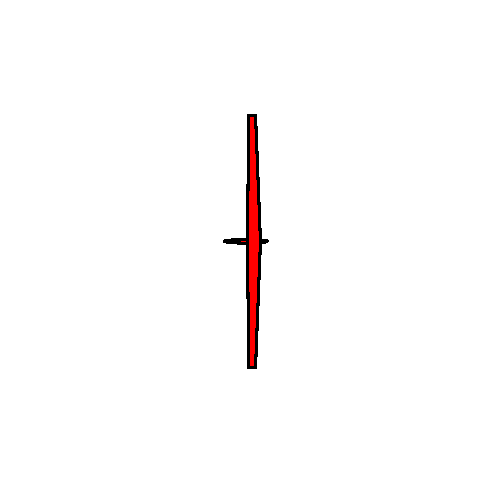
\includegraphics[trim={9.5cm 1cm 9.5cm 1cm},clip,height=3.8cm]{box.eps} &
    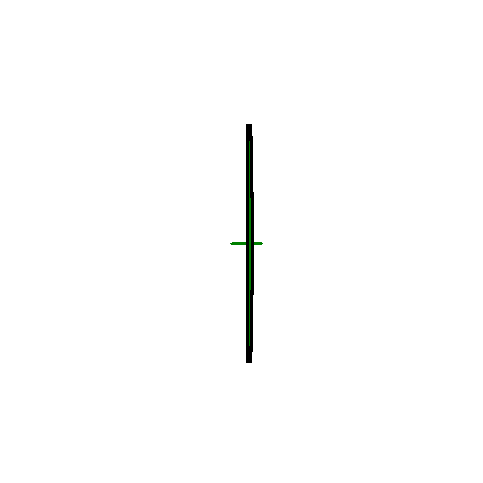
\includegraphics[trim={9.5cm 1cm 9.5cm 1cm},clip,height=3.8cm]{elliptical.eps} \\
\hline
Objective metric & Description & Units & No Uncert. & Margins & Box & Elliptical \\
\hline
Objective & total fuel weight & $\mathrm{N}$ & 612 & 1182 & 1252 & 1098 \\
E[Objective] & expected total fuel weight & $\mathrm{N}$ & 591 & 982 & 993 & 871 \\
$\sigma$[Objective] & std. dev. of fuel weight & $\mathrm{N}$ & 9 & 32 & 32 & 29 \\
P[failure] & probability of failure & \% & 94 & 0 & 0 & 0\\
\hline
\end{tabular}
\end{center}
\end{table}

It is noteworthy in the probability of failure at the bottom of Table~\ref{tab:results} that,
for the nominal problem ($\Gamma = 0$),
only 6 percent of the \gls{mc} evaluations result in feasible solutions.
This means that an aircraft designed for the average case would almost surely
fail to satisfy the mission requirements, even with equal likelihood of favorable versus
unfavorable uncertain outcomes from the symmetric truncated Gaussian.
That being said, depending on the problem, it may necessary to sacrifice
performance to achieve a high degree ($3\sigma$) of
reliability as in the solution for $\Gamma = 1$. Furthermore, the margin aircraft, the box aircraft
and the elliptical aircraft spend on average 66\%, 68\% and 47\% more fuel respectively
than the aircraft designed for the nominal case, but they also are
robust to all uncertain outcomes in the $3\sigma$ set for the given \gls{mc} simulation.

Table~\ref{tab:results} also indicates that margins are not a good method of
allocating uncertainty. The claim for the use of margins is that they protect against
the worst case outcome of each parameter, but the results show otherwise.
Since the box design at $\Gamma=1$ is strictly
more conservative (worse worst-case outcome) over the $3\sigma$ hypercube
than the margin design, we see that a margin from the interior of the hypercube
rather than its corner is more effective in protecting against the worst case.
Furthermore, there are no probabilistic
guarantees that the aircraft
with margins would not fail one of the \gls{mc} simulations. Given enough samples,
it is almost surely true that some \gls{mc} simulations will violate feasibility
for the design with margins,
whereas box uncertainty guarantees deterministically that the constraints are satisfied.

We also posited that the elliptical uncertainty, although it doesn't
protect deterministically against all $3\sigma$ uncertainties, would be less conservative than the
margin and box designs while not significantly sacrificing probability of failure. This is
confirmed since the elliptical design fails none of the random samples,
and spends 11 and 12\% less fuel on average
than the margin and box aircraft respectively.
The significance of this cannot be understated: the use of elliptical uncertainty
results in designs that have strictly better performance outcomes, while protecting
against a similar amount of risk as designs using margins or box uncertainty.

\begin{figure}[ht]
    \centering
    \captionsetup{justification=centering, font=small}
    \begin{subfigure}{0.49\textwidth}
        \centering
        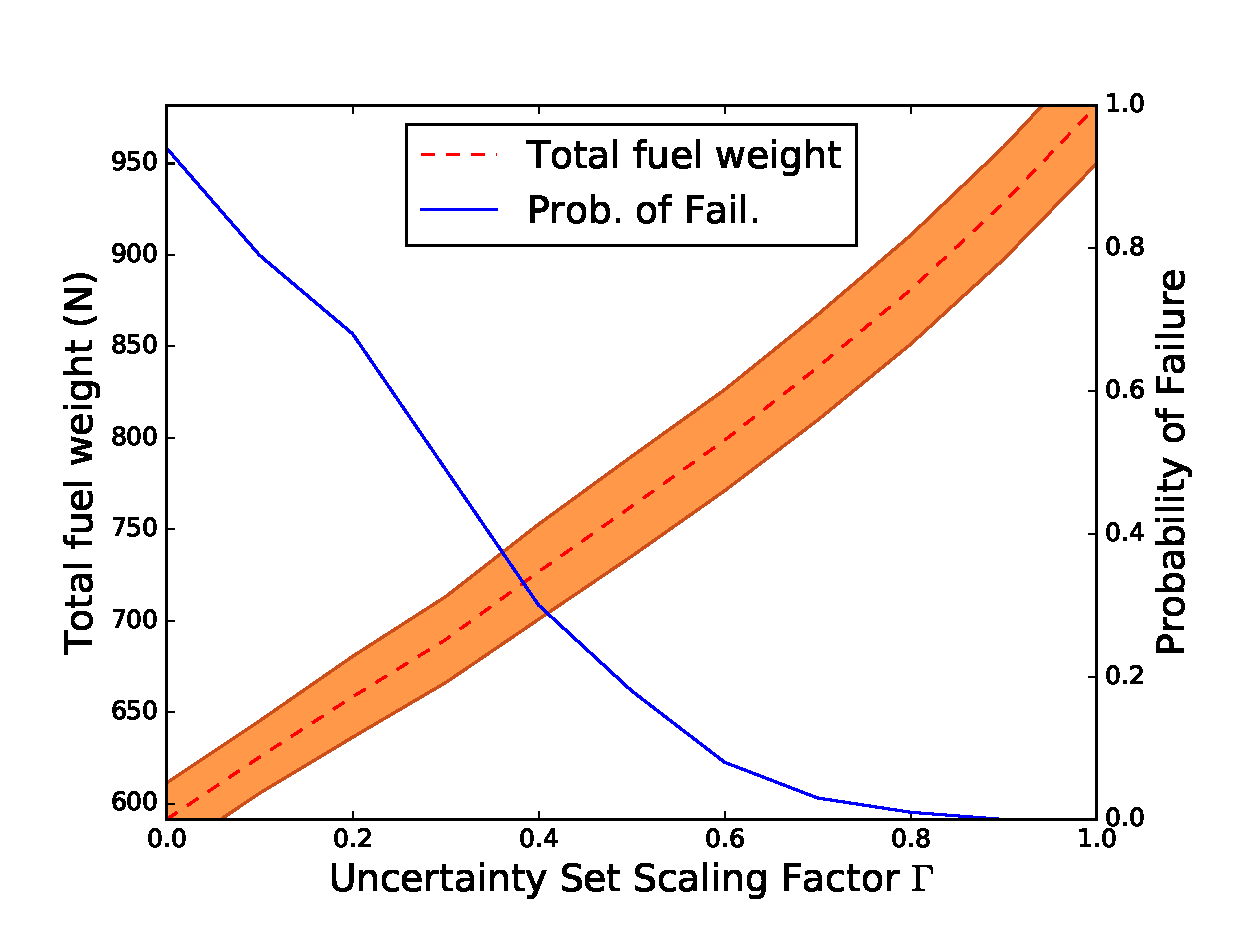
\includegraphics[height=2.3in]{marginspof.eps}
         \caption{Margins}
    \end{subfigure}%
    \begin{subfigure}{0.49\textwidth}
        \centering
        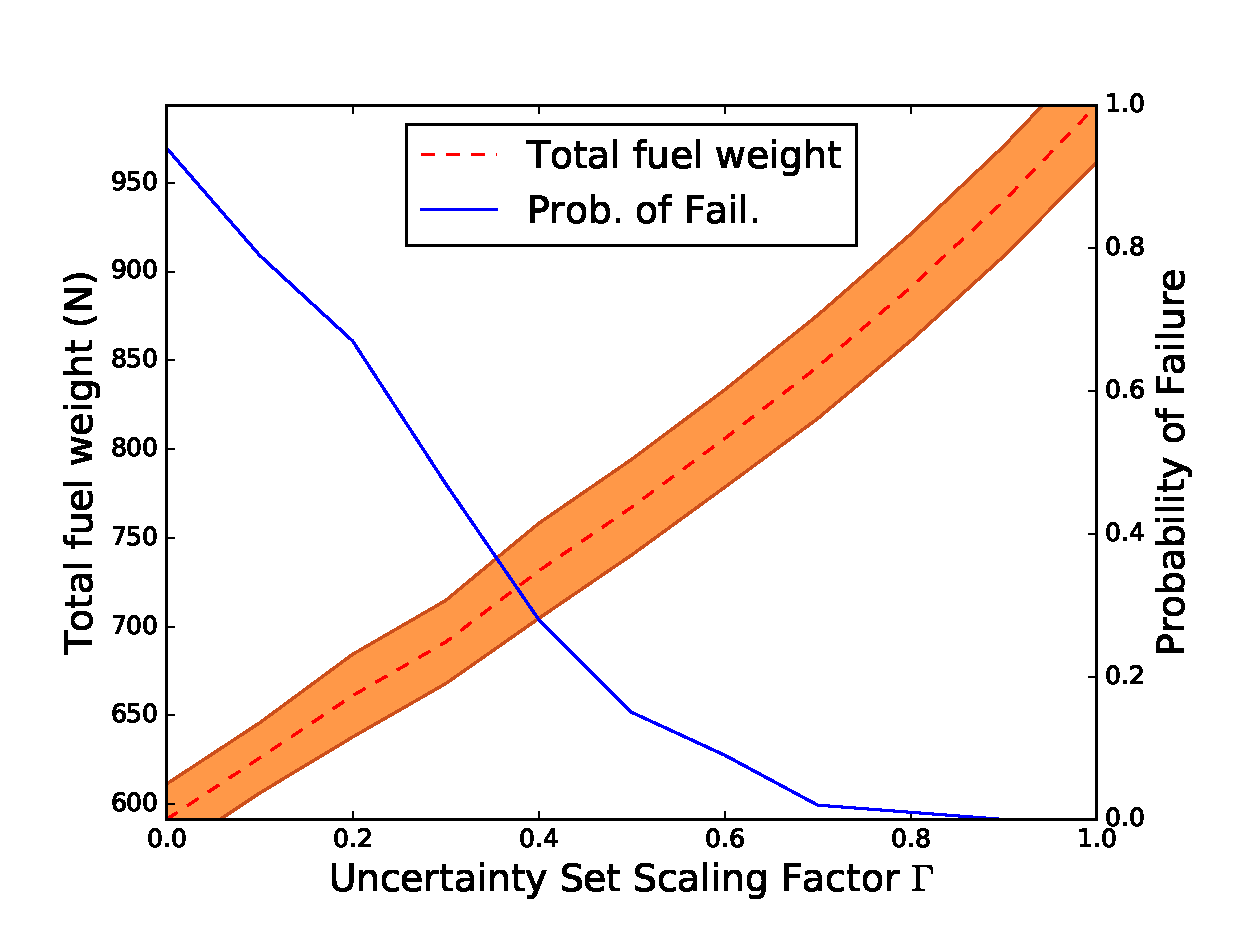
\includegraphics[height=2.3in]{box_best_pairs.eps}
         \caption{Box Uncertainty Set}
    \end{subfigure}%
    \\
    \begin{subfigure}{0.49\textwidth}
        \centering
        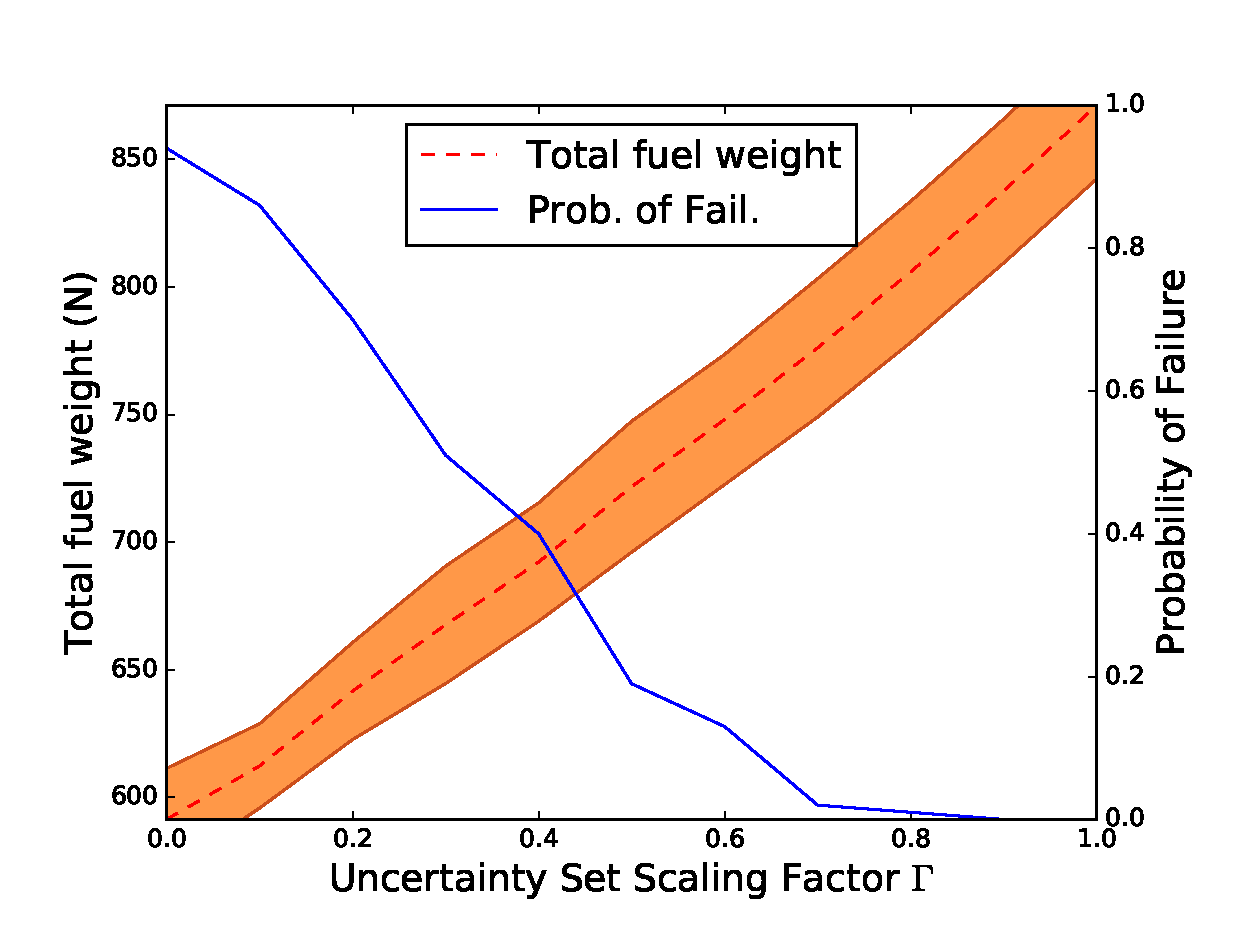
\includegraphics[height=2.3in]{ell_best_pairs.eps}
         \caption{Elliptical Uncertainty Set}
    \end{subfigure}
    \caption{Simulated performance of the optimal robust aircraft, using margins, box and elliptical uncertainty sets,
    as a function of $\Gamma$. The robust solutions use the Best Pairs formulation.
    The dashed line and the band represent the mean and standard deviation of the performance
    of aircraft, simulated with 100 \gls{mc} samples of uncertain parameters.}
    \label{fig:probOfFailure}
\end{figure}

An analysis on the range $\Gamma=[0,1]$ was performed to confirm that the trends from
Table~\ref{tab:results} hold for all $\Gamma$. Figure~\ref{fig:probOfFailure}
shows that probability of failure goes monotonically
towards zero as $\Gamma$ increases for all three methods, where box uncertainty is
more conservative than margins, and elliptical uncertainty is less conservative
than the other two methods over the whole $\Gamma$ domain.

\begin{figure}[h!]
    \centering
    \captionsetup{justification=centering, font=small}
    \begin{subfigure}{0.49\textwidth}
        \centering
        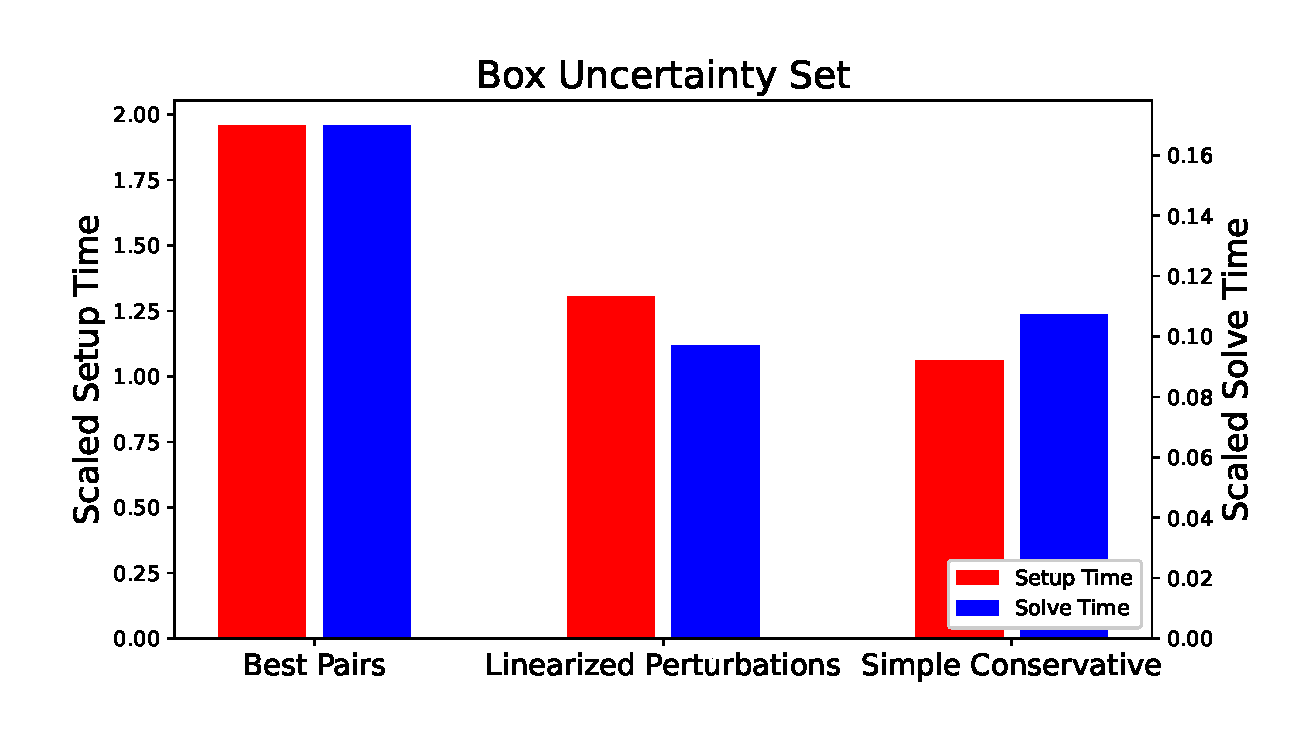
\includegraphics[height=1.9in]{box_sst.eps}
    \end{subfigure}
    ~
    \begin{subfigure}{0.49\textwidth}
        \centering
        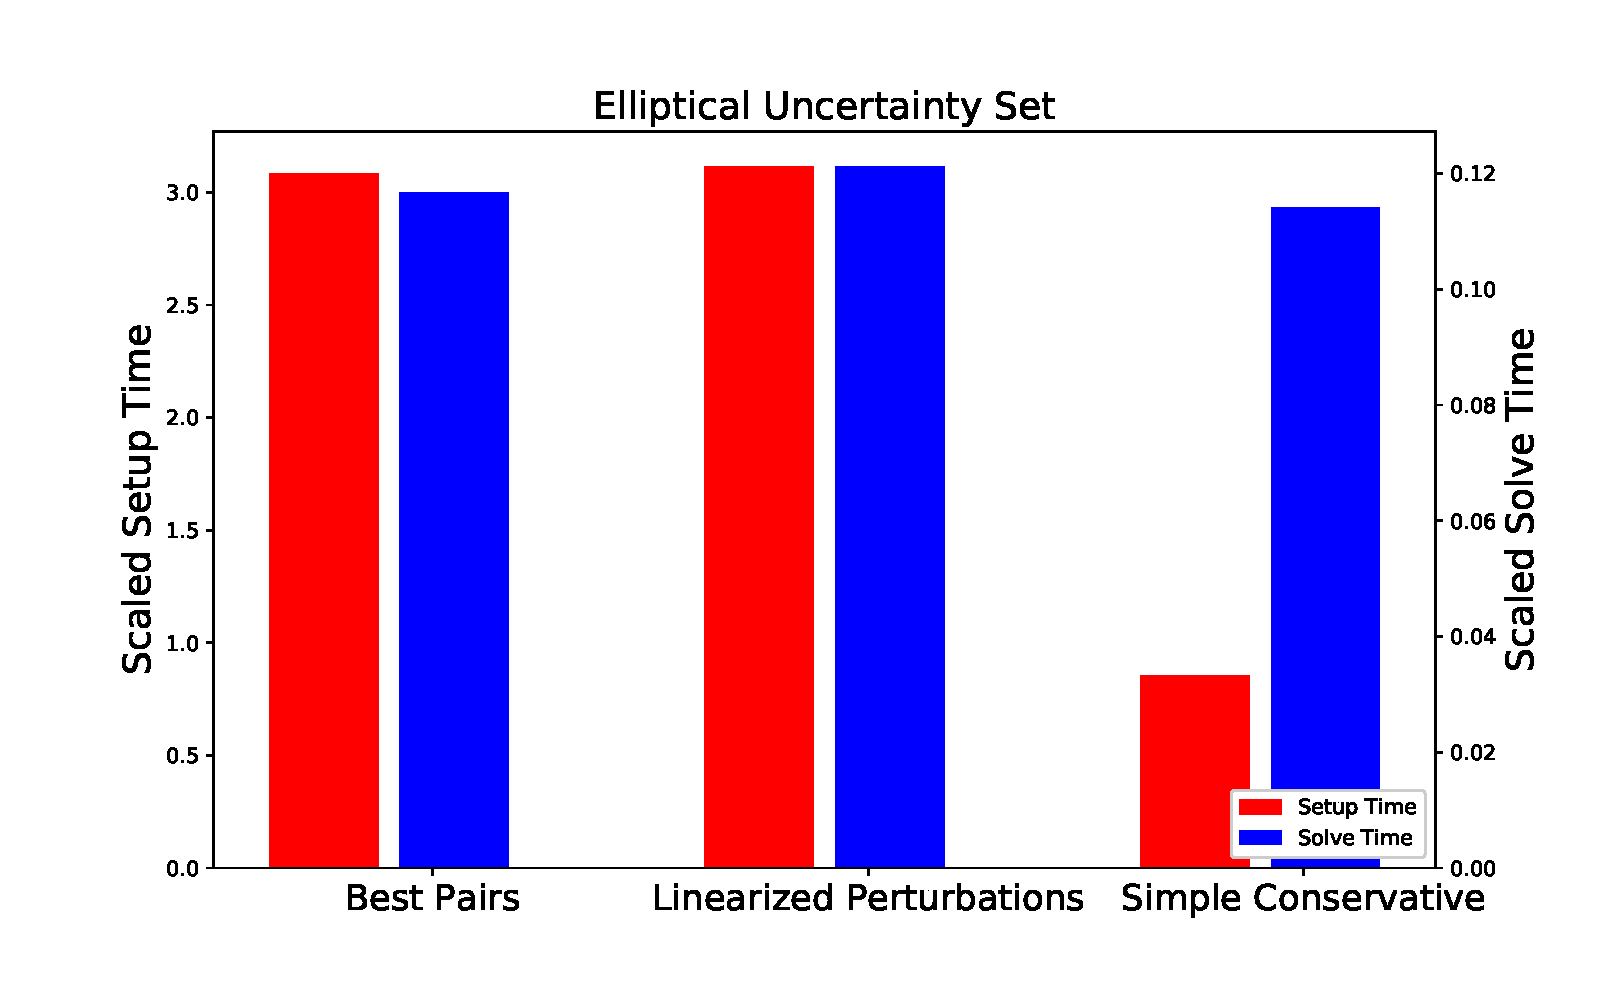
\includegraphics[height=1.9in]{ell_sst.eps}
    \end{subfigure}
    \caption{Robust signomial simple aircraft solution and setup times, normalized by the
    nominal problem solution time, for $\Gamma = 1$.
    Note that the problems with box uncertainty have lower setup
    time costs versus those with elliptical uncertainty, but similar solve times.}
    \label{compare_signomial}
\end{figure}

In absolute
terms, the nominal \gls{sp} under zero uncertainty or with margins
takes just under 0.9 seconds to solve on a modern laptop computer using Mosek~\cite{mosek},
an interior point solver that is free for academic use; the authors
refer to ~\cite{Kirschen2018Log} and \cite{York2018} for more in-depth \gls{sp} solution time analyses.
Here we examine briefly in relative terms about how the different \gls{rsp} methodologies compare in terms of setup and
run times in Figure~\ref{compare_signomial}. Since the setup time of the nominal problem is minimal,
we have normalized the results by the solution time of the nominal problem.
The bottom axis ranks the methods by their level of conservativeness, Best Pairs
and Simple Conservative formulations being the least and most conservative respectively,
and where the elliptical formulations are less conservative than the box formulations.
For this aircraft design problem, the preferred Best Pairs methodology
is competitive in solution and setup times for both types of uncertainty set. Furthermore
the box uncertainty set generally requires lower setup time (other than the Simple Conservative case)
than the elliptical uncertainty set.
Note that setup and solution times for \gls{rsp}s are highly problem-specific, so it is not possible
to predict the time performance of other \gls{rsp}-compatible problems from these results.
Time performance will vary depending on the number of inequality constraints,
the degree of coupling between monomials
in each inequality, and the \gls{rgp} approximation and uncertainty set used.

\subsection{The Effect of Robustness on Multiobjective Performance}

One of the benefits of convex and difference-of-convex optimization methods is the ability to optimize for
different objectives~\cite{York2018}. As a demonstration, we optimize the aircraft without uncertainty
for 8 different objectives, and show
the non-dimensionalized figures of merit in the columns of Table~\ref{tab:nondimresults}.
Since the model is physics based, the model can even accommodate objectives such as aspect ratio
which are unintuitive and often not considered. The resulting aircraft
differ drastically with respect to performance.
As an extreme example,
the aircraft optimized for time cost has nearly 200 times the engine weight as the aircraft
optimized for total fuel, since drag power increases dramatically with speed. Furthermore, we can see
that some more traditional objectives such as wing loading pull the design
towards extreme corners of the performance envelope. This shows the importance of considering many objectives
in design, and demonstrates the power of \gls{sp}s in helping
consider the multiobjective performance of engineered systems.

\begin{table}
\resizebox{\textwidth}{!}{
\begin{tabular}{C{2.2cm} | C{1.5cm} C{1.5cm} C{1.5cm} C{1.5cm} C{1.5cm} C{1.5cm} C{1.5cm} C{1.5cm}} 
Objective & Total fuel & Time cost & Total cost & Takeoff weight & 1/(Cruise L/D) & Aspect ratio & Engine weight & Wing loading \\ \hline
Total fuel & 1.00 & 1.00 & 1.00 & 1.00 & 1.00 & 1.00 & 1.00 & 1.00 \\ 
Time cost & 13.48 & 0.32 & 3.00 & 3.88 & 11.18 & 0.13 & 193.89 & 1.00 \\
Total cost & 1.54 & 0.55 & 0.75 & 0.93 & 1.54 & 0.48 & 4.55 & 1.00 \\
Takeoff weight & 1.32 & 0.79 & 0.90 & 0.85 & 1.38 & 0.35 & 2.03 & 1.00 \\
1/(Cruise L/D) & 1.27 & 0.96 & 1.02 & 1.13 & 0.81 & 0.92 & 4.84 & 0.76 \\
Aspect ratio & 15.21 & 0.65 & 3.61 & 3.33 & 16.82 & 0.02 & 102.82 & 0.37 \\
Engine weight & 1.25 & 1.46 & 1.42 & 1.21 & 1.38 & 1.06 & 0.76 & 0.63 \\
Wing loading & 32.80 & 2.00 & 8.26 & 17.04 & 35.27 & 0.19 & 62.61 & 0.11 \\
\hline
\end{tabular}}
\caption{Non-dimensionalized variations in objective values with respect to the aircraft optimized
for different objectives. Objective values are normalized by the total fuel solution.}
    \label{tab:nondimresults}
\end{table}

Aside from this caricature example, we demonstrate the capabilities of \gls{rsp}s
by considering a more realistic scenario, now with uncertainty.
We perform the optimization of the aircraft with no uncertainty, and both box and
ellipsoidal uncertainty ($\Gamma = 1$)
for 4 different objective functions, and plot the results on radar plots.
Radar plots are useful because they allow engineers to visualize the performance
of designs in many dimensions. One way to envision the multi-objective
performance of the aircraft is to consider the area of the polygon defined by the aircraft's
performance as the figure of merit; the smaller the better.
Due to the large disparities in the figures of merit depending on the objective function choice
in Table~\ref{tab:nondimresults}, we choose to demonstrate this using four objective functions
that would traditionally be used in aircraft design, and be expected to have a high degree of correlation.
These are total (time and fuel) cost, total fuel, takeoff weight and inverse cruise lift-over-drag (L/D).

\begin{figure}[!ht]
    \begin{center}
    \begin{tikzpicture}
        \node[inner sep=0] (center) at (0,0)
        {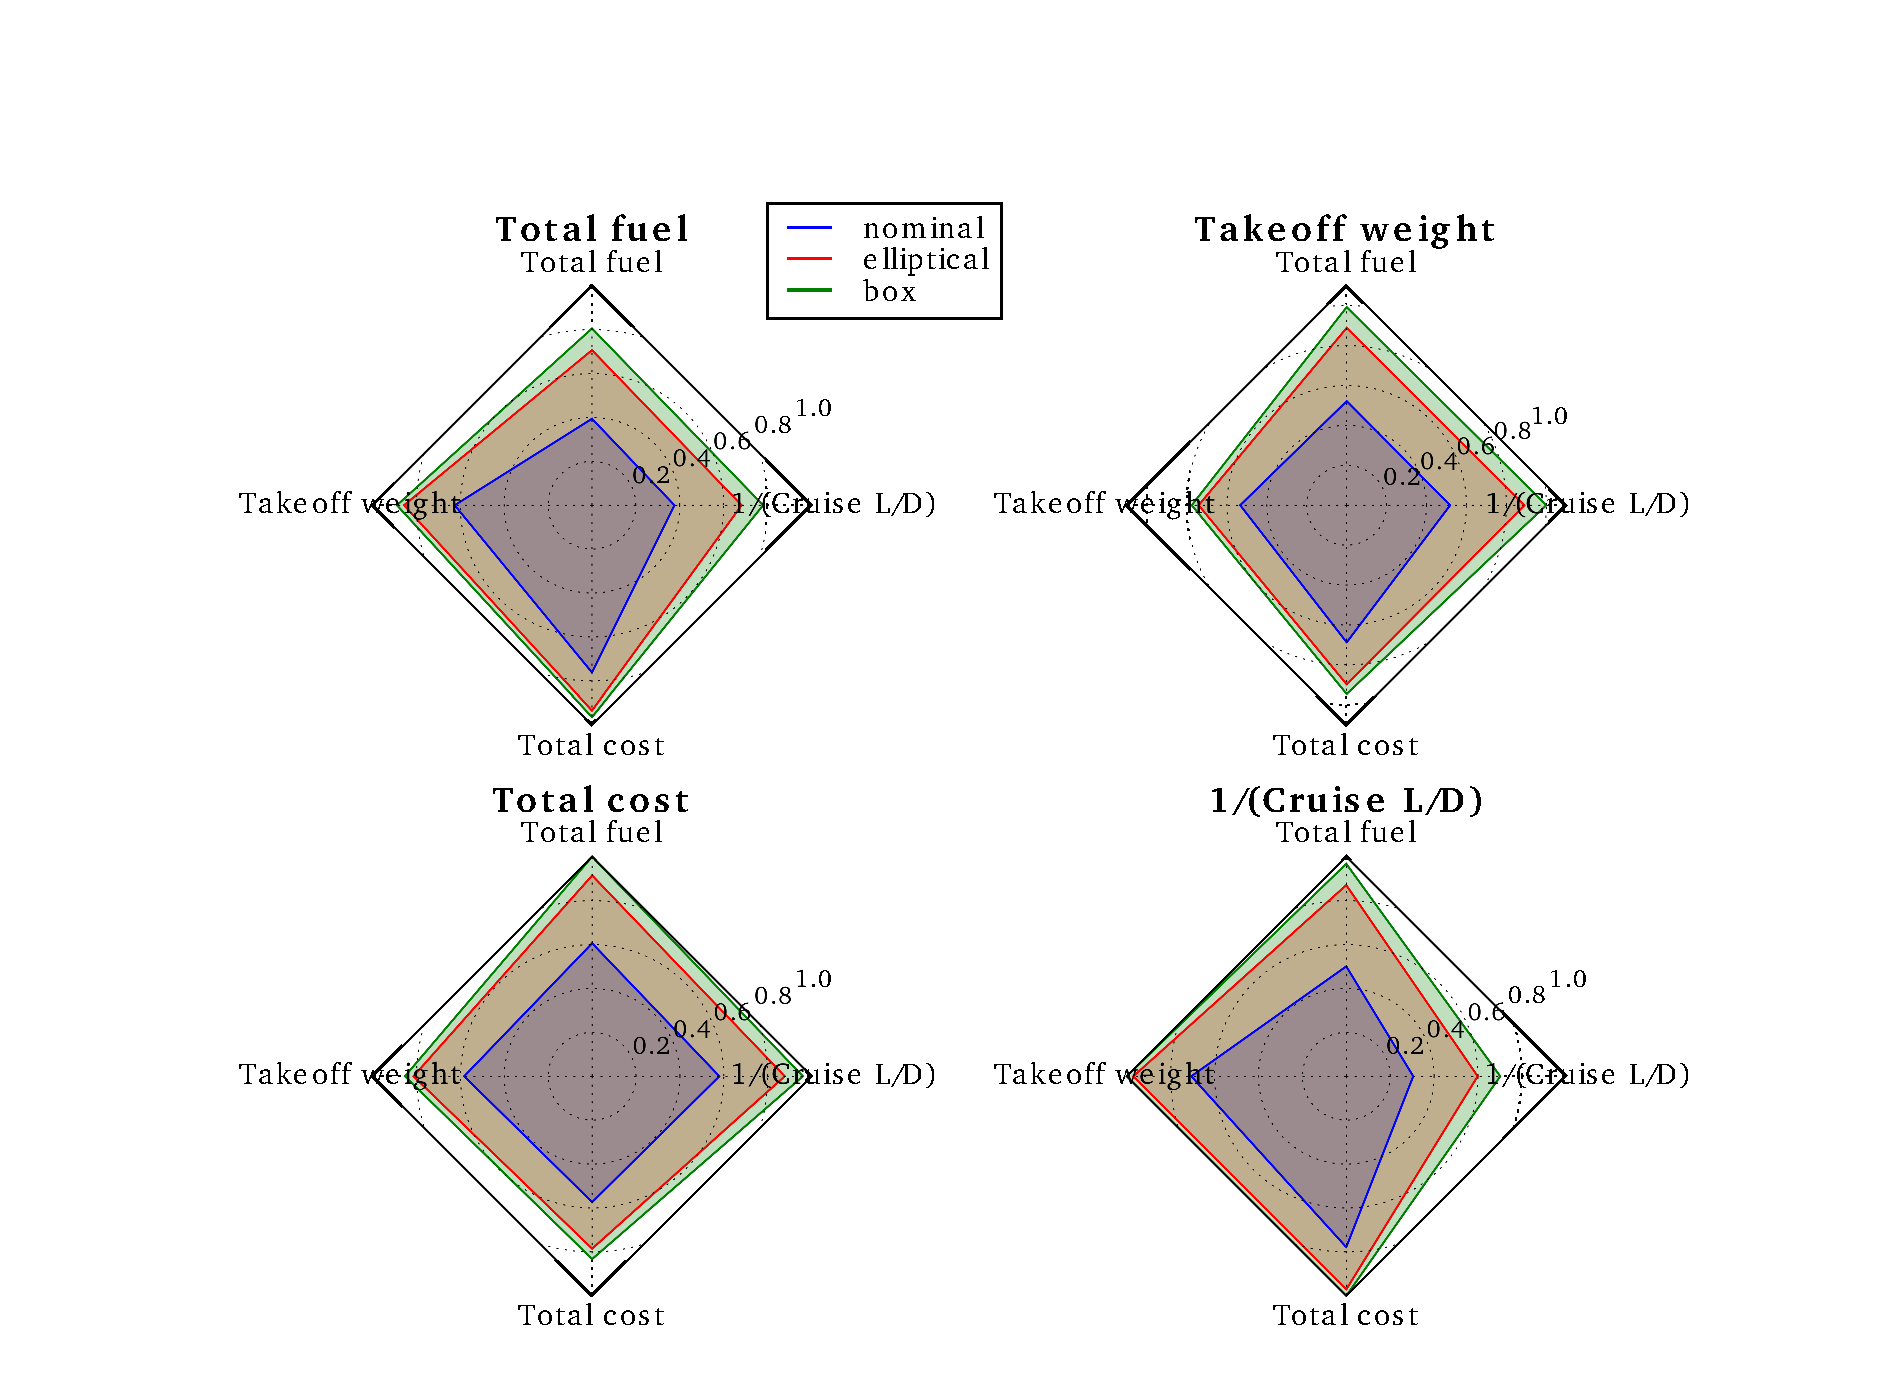
\includegraphics[trim={2cm 0 1cm 0},clip,scale=0.6]{4objradar.eps}};
        \node[inner sep=0] (ul) at (-1.0, 0.25)
        {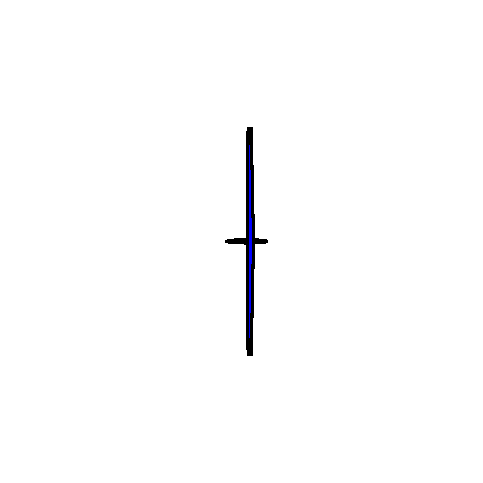
\includegraphics[height=3.8cm]{0nominal.eps}};
        \node[inner sep=0] (ur) at (1.0, 0.25)
        {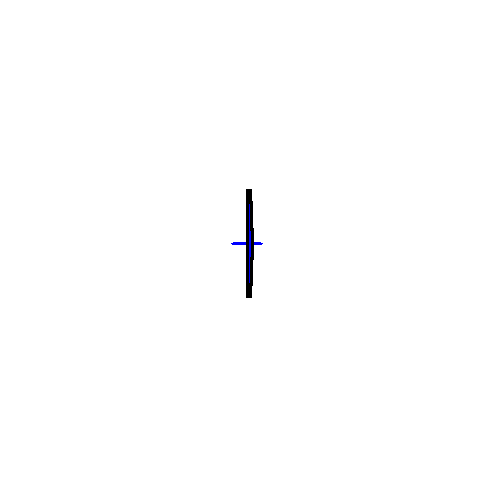
\includegraphics[height=3.8cm]{1nominal.eps}};
        \node[inner sep=0] (ll) at (-1.0, -2)
        {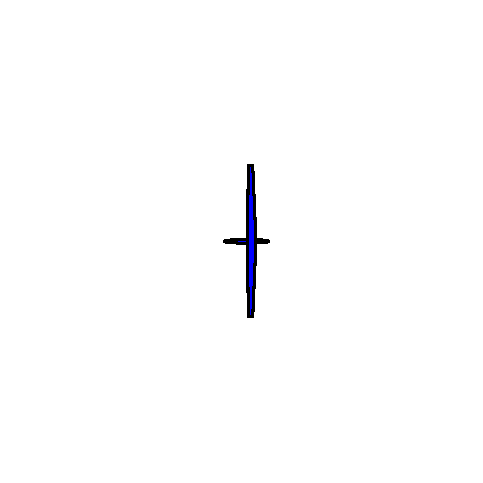
\includegraphics[height=3.8cm]{2nominal.eps}};
        \node[inner sep=0] (lr) at (1.0, -2)
        {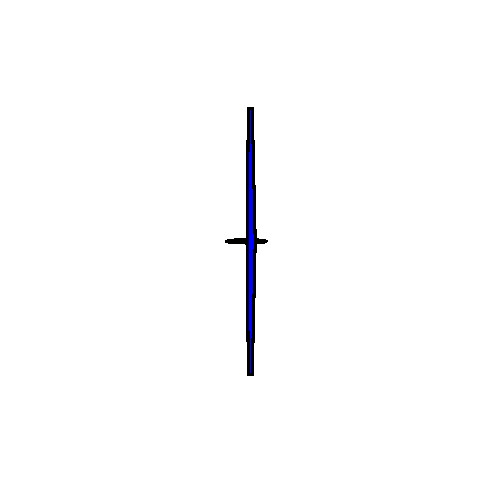
\includegraphics[height=3.8cm]{3nominal.eps}};
    \end{tikzpicture}
    \caption{The radar plots of aircraft performance, for aircraft optimized for different objectives.
    The bolded titles are the design objectives for each plot, whereas the individual plots
    show the non-dimensionalized multiobjective performance of the aircraft designed under different
    uncertainty sets. Nominal aircraft sketched for comparison. }
    \label{fig:radar}
\end{center}
\end{figure}

\begin{figure}
    \begin{center}
        \begin{subfigure}{0.4\linewidth}
            \makebox[\textwidth]{\begin{tikzpicture}
                \node[inner sep=0] (l) at (-2.5,0)
                {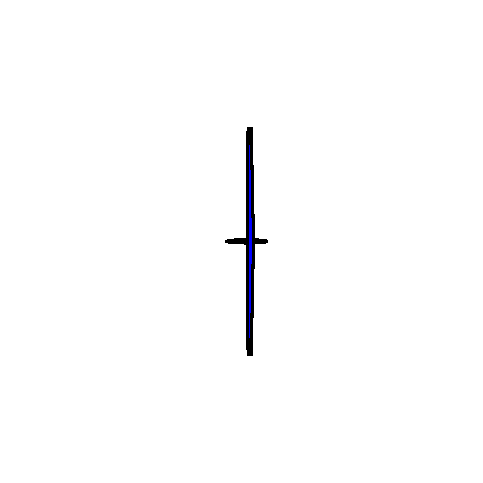
\includegraphics[trim={9.5cm 1cm 8.5cm 1cm},clip,height=3.8cm]{0nominal.eps}};
                \node[inner sep=0] (c) at (-1,0)
                {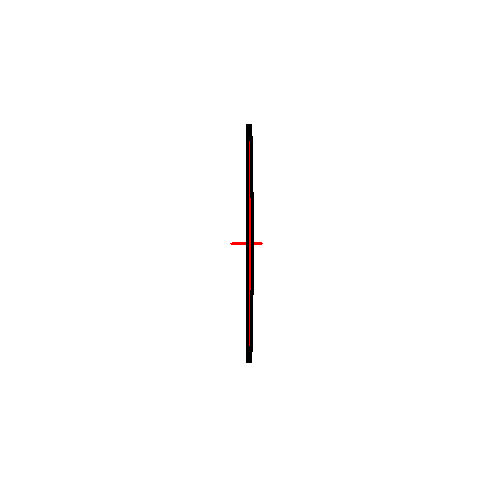
\includegraphics[trim={9.5cm 1cm 8.5cm 1cm},clip,height=3.8cm]{0elliptical.eps}};
                \node[inner sep=0] (r) at (.5,0)
                {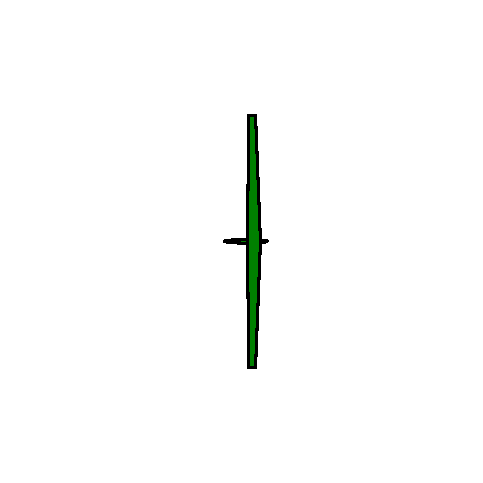
\includegraphics[trim={9.5cm 1cm 8.5cm 1cm},clip,height=3.8cm]{0box.eps}};
            \end{tikzpicture}}
            \caption{Total fuel}
        \end{subfigure}
        \begin{subfigure}{0.4\linewidth}
            \makebox[\textwidth]{\begin{tikzpicture}
                \node[inner sep=0] (l) at (-2.5,0)
                {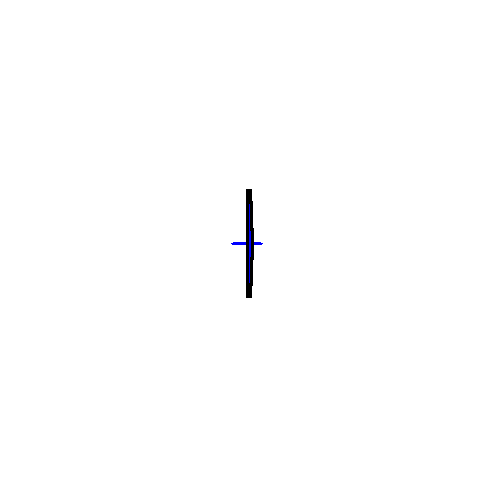
\includegraphics[trim={9.5cm 1cm 8.5cm 1cm},clip,height=3.8cm]{1nominal.eps}};
                \node[inner sep=0] (c) at (-1,0)
                {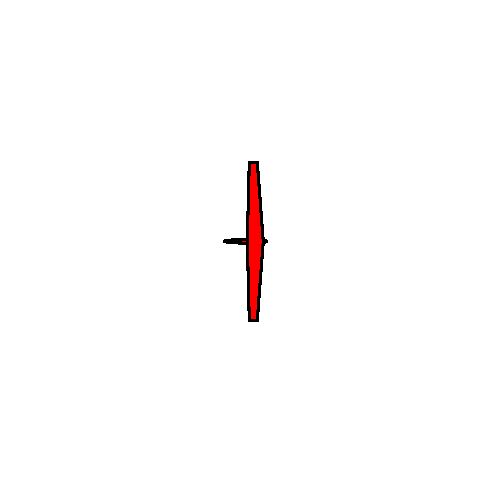
\includegraphics[trim={9.5cm 1cm 8.5cm 1cm},clip,height=3.8cm]{1elliptical.eps}};
                \node[inner sep=0] (r) at (.5,0)
                {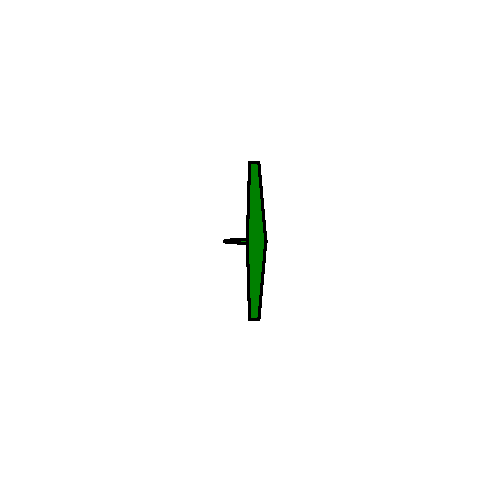
\includegraphics[trim={9.5cm 1cm 8.5cm 1cm},clip,height=3.8cm]{1box.eps}};
            \end{tikzpicture}}
            \caption{Takeoff weight}
        \end{subfigure}
        \begin{subfigure}{0.4\linewidth}
            \makebox[\textwidth]{\begin{tikzpicture}
                \node[inner sep=0] (l) at (-2.5,0)
                {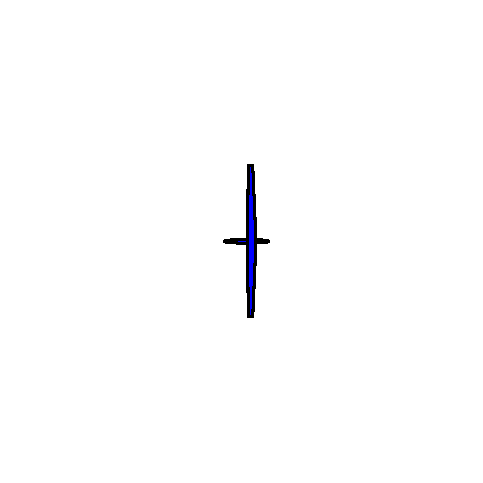
\includegraphics[trim={9.5cm 1cm 8.5cm 1cm},clip,height=3.8cm]{2nominal.eps}};
                \node[inner sep=0] (c) at (-1,0)
                {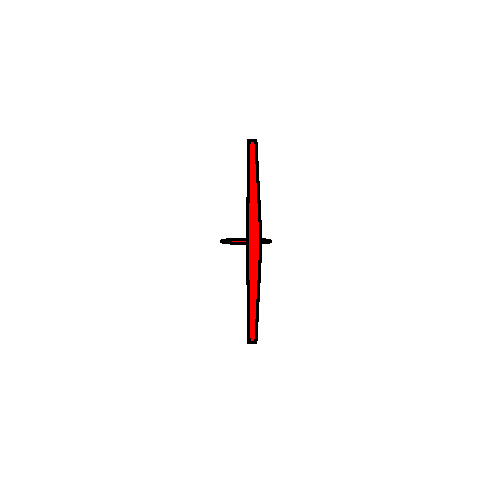
\includegraphics[trim={9.5cm 1cm 8.5cm 1cm},clip,height=3.8cm]{2elliptical.eps}};
                \node[inner sep=0] (r) at (.5,0)
                {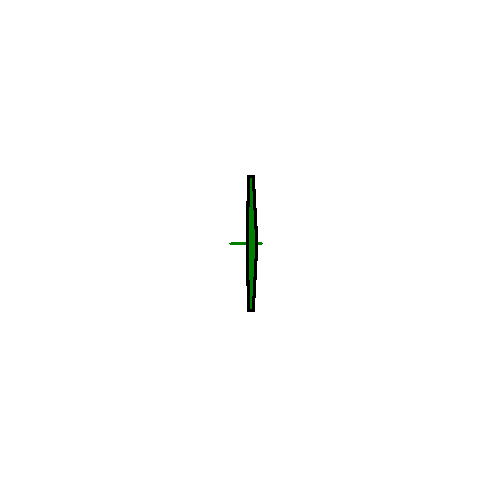
\includegraphics[trim={9.5cm 1cm 8.5cm 1cm},clip,height=3.8cm]{2box.eps}};
            \end{tikzpicture}}
            \caption{Total cost}
        \end{subfigure}
        \begin{subfigure}{0.4\linewidth}
            \makebox[\textwidth]{\begin{tikzpicture}
                \node[inner sep=0] (l) at (-2.5,0)
                {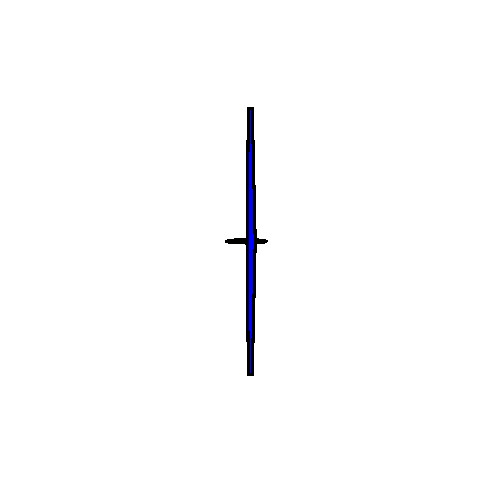
\includegraphics[trim={9.5cm 1cm 8.5cm 1cm},clip,height=3.8cm]{3nominal.eps}};
                \node[inner sep=0] (c) at (-1,0)
                {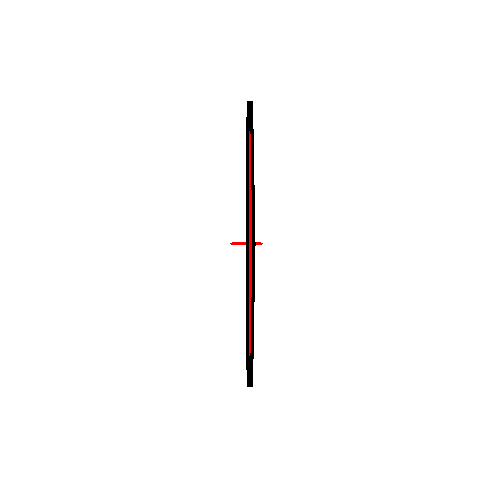
\includegraphics[trim={9.5cm 1cm 8.5cm 1cm},clip,height=3.8cm]{3elliptical.eps}};
                \node[inner sep=0] (r) at (.5,0)
                {
\includegraphics[trim={9.5cm 1cm 8.5cm 1cm},clip,height=3.8cm]{3box.eps}};
            \end{tikzpicture}}
            \caption{1/(Cruise L/D)}
        \end{subfigure}
        \caption{Sketches of the aircraft drawn for corresponding radar plots. Drawn to scale for comparison.}
    \end{center}
\end{figure}

Figure~\ref{fig:radar} shows the effects of robustness on
the different worst-case performance metrics of the different aircraft.
As expected, the box uncertainty set is strictly more conservative than the elliptical uncertainty set for
all objectives. Note that the radar plots show the worst-case performance of the vehicles, although
this analysis can also be performed for the mean performance
of the aircraft determined through ~\gls{mc} simulation.

This multiobjective comparison underscores the importance of optimization under uncertainty
in conceptual design especially when multiple, potentially conflicting objectives are present.
If the inverse cruise L/D solution
on the lower-right of Figure~\ref{fig:radar} is compared with the nominal total fuel solution on the upper-left, their
performance profiles are similar. When parametric uncertainty is added however, we see that aircraft
that maximize cruise L/D perform badly in the worst-case
in all other objectives. This means that robust requirements can
affect the efficacy of different objective functions in ensuring multiobjective performance.
Since \gls{rsp}s can be solved quickly and reliably over a variety of objective functions,
they allow engineers to understand these kinds of complex trade-offs early on in the design process.

Based on these observations, we argue that there could be significant value left on the table
if uncertainty is not considered with sufficient mathematical rigor in early phases of
the design process. \gls{rsp}s allow engineers to capture complex
trade-offs in nonlinear optimization problems while considering uncertainty,
resulting in \emph{less conservative} solutions
than solutions that implement margins and other less mathematically
rigorous methods for risk mitigation.
Thus \gls{rsp}s improve significantly on the
the paradigms of design under uncertainty in use
in the aerospace industry today.

\subsection{Risk minimization problems}

All of the previous multi-objective analyses have assumed that we have an
understanding of exactly the amount of uncertainty we are
willing to tolerate. However, minimizing risk can also be the objective of our
model. This would suggest the following formulation:
\begin{equation}
    \begin{split}
    \text{max}~~\Gamma \\
    \text{s.t.}~~f_i(x,u) &\leq 0,~i = 1,\ldots,n \\
                    \left\lVert u \right\rVert &\leq \Gamma \\
                    f_0(x) &\leq (1+\delta)f_0^*,~\delta \geq 0
    \end{split}
    \label{eq:goalprogramming}
\end{equation}
where $f_0^*$ is the optimum of the nominal problem in Formulation~\ref{eq:normform} and $\delta$
is a fractional penalty on the objective that we are willing to sacrifice for robustness, which
gives $(1+\delta)f_0^*$ as the upper bound on the objective value. Intuitively,
this is a form of goal programming,
where we specify the exact maximum worst-case value of an objective we can tolerate with
the goal of maximizing the total size of the uncertainty $\Gamma$ we can handle.

The goal programming problem in Formulation~\ref{eq:goalprogramming} is clearly
not equivalent to the problem in Formulation~\ref{eq:normform},
but should yield the same results if both methods are optimal.
To show this, we use the worst-case objective values from the probability of failure study
shown in Figure~\ref{fig:probOfFailure} as the $\delta$ inputs to the goal programming model, and compare the results.
The results are presented in
Table~\ref{tab:deltaVsGamma}. Note that the two methods were evaluated \gls{mc} runs using the same 100 realizations
of the uncertainty, for consistency in probability of failure results.

\begin{table}
\begin{center}
\caption{\label{tab:deltaVsGamma} Results of original \gls{ro} problem versus goal program in terms
of size of uncertainty set $\Gamma$, objective penalty $\delta$, and probability of failure. Both methods
use the Best Pairs formulation under elliptical uncertainty. The designs obtained through
the two different methods match.}
\begin{tabular}{c c c c c c c c}
\hline
 \gls{ro} form & $\Gamma$ & $\delta$ & PoF & Goal form & $\delta$ & $\Gamma$ & PoF\\
\hline
& 0.00 & $1.66 \times 10^{-4}$ & 0.94 & & $1.66 \times 10^{-4}$ & - & - \\
& 0.10 & 0.0574 & 0.86 & & 0.0574 & 0.10 & 0.86 \\
& 0.20 & 0.119 & 0.70 & & 0.119 & 0.20 & 0.70 \\
& 0.30 & 0.184 & 0.51 & & 0.184 & 0.30 & 0.51 \\
& 0.40 & 0.254 & 0.28 & & 0.254 & 0.40 & 0.28 \\
& 0.50 & 0.328 & 0.19 & & 0.328 & 0.50 & 0.20 \\
& 0.60 & 0.409 & 0.13 & & 0.409 & 0.60 & 0.13 \\
& 0.70 & 0.495 & 0.02 & & 0.495 & 0.70 & 0.02 \\
& 0.80 & 0.587 & 0.01 & & 0.587 & 0.80 & 0.01 \\
& 0.90 & 0.686 & 0.00 & & 0.686 & 0.90 & 0.00 \\
& 1.00 & 0.793 & 0.00 & & 0.793 & 1.00 & 0.00 \\
\end{tabular}
\end{center}
\end{table}

Firstly, note that there are no results reported for the goal program
for zero uncertainty, $\Gamma = [0.00]$.
Since the feasible set of this problem is a point design, the signomial program
solution heuristic declares the problem infeasible after being
unable to locate the singular feasible region. However when we positively perturb
the singular $\delta$, the goal program has a non-empty feasible set and
returns the same solution as the original \gls{ro} method.
Otherwise, the $\Gamma$ values found by the goal program match exactly
with the original \gls{ro} problem. We confirm that both methods produce
the same designs by examining the physical dimensions of the aircraft, and through the probability
of failure found through \gls{mc} simulation in Table~\ref{tab:deltaVsGamma}.
Note that there is a small discrepancy
in the probability of failure, notably in the value for $\Gamma = 0.5$. This is
possible because there are uncertainty realizations that can fall
in or out of feasibility due to numerical precision. The interior point solvers
used cannot make computations exactly~\cite{Nesterov1994}.

We can also expand this framework to perform multivariate goal programming,
by changing Formulation~\ref{eq:goalprogramming} to include all
objectives we are interested in.
\begin{equation}
    f_{0,j}(x) \leq (1+\delta_j) f^*_{0,j},~\delta_j \geq 0,~j = 1,\ldots, m
    \label{eq:multigoal}
\end{equation}

The benefit of goal programming is that it allows us to explore multidisciplinary trade-offs without
having to enumerate the design space along each objective direction.
The term multiobjective optimization is misleading
because you can only optimize for one objective at once.
The design is going to be influenced by how engineers weigh different objectives, and
it is not obvious whether an objective should be a constraint instead. The most
fundamental choice that an engineer can make in design is what the objective function is, and it is
often the case that there are many potential objectives that are conflicting.
But risk is ubiquitous in engineering design problems, so goal programming allows risk to be used as
a global design variable against which all objectives can be weighed.

\section{Potential Future Work or Studies}

There are a myriad of potential extensions to signomial programming under uncertainty.
In the spirit of helping reduce program risk in aerospace design,
the authors make a few observations and recommendations.

In this study, we do not discriminate between the kinds of constraints violated. However, it would
be possible to rank the severity of constraint violations so as to penalize some (eg. structural safety)
more heavily than others (maximum range constraint). This would inject further realism into
design under uncertainty since some violations contribute to program risk more
significantly than others.

Another potentially valuable extension to the proposed framework is the concurrent implementation
of multiple sets to contain the uncertain parameters, with the purpose of restricting uncertain
outcomes further and reducing conservativeness.
One example of this would be to impose an  L1-norm on the integer number of uncertain parameters
as well as an L2-norm on the overall size of uncertainty set.
This method can be used to set the total size of the uncertainty set in a Euclidian sense,
but then also to restrict the uncertainty to a subset of all of the uncertain parameters.
This also turns the problem into an integer robust
optimization problem which poses interesting computational challenges.

With respect to interesting studies, \gls{ro} opens up the possibility to discover and analyze
with mathematical rigor the benefits
of adaptable architectures in aircraft design versus more traditional point designs.
Some examples of these are modular designs, morphing designs,
adaptively manufactured designs and aircraft families. It is likely that these types of engineered
robustness become more effective at reducing program risk
in presence of uncertainty, since they are more likely
to deliver value under adverse stochastic outcomes.

In situations where there is data available to aid design, \gls{ro} can help explore
the design space while taking into account the sparsity of and noise in the data.
This opens up an array of potential trade studies where engineers can learn about
the exposure of designs to the quality of data and attempt to gather
data which best reduces the uncertainty in the performance of designs.
